\section{Introduction}
\label{sec:intro}

With the discovery of a new scalar particle the Higgs boson~\cite{HIGG-2012-27,CMS-HIG-12-028} at the LHC~\cite{Evans:2008zzb} by the ATLAS and CMS collaborations with a mass of 125 GeV~\cite{HIGG-2016-33,HIGG-2013-12,HIGG-2014-14,CMS-HIG-14-009}, the whole content of the Standard Model (SM) of particle physics became complete. A priority of the ATLAS and CMS collaborations has been to better understand its properties and couplings.
After the EWSB and the higgs field acquires the vev, the higgs potential obtained in Equation.. can be obtained as following:
\begin{align}
	V(\phi) \rightarrow V(\phi)_{\text{EWSB}} =  -\lambda \nu^2 h^2 - \lambda \nu h^3 - \frac{1}{4} \lambda h^4 + \text{const.}
	\label{eq:higgs_pot}
\end{align}
The first term of the above equation is the Higgs mass term, and the remaining are the trilinear and quadri-linear Higgs-self couplings,
\begin{align}
	\underbrace{m_{h} = \sqrt{ - 2 \mu^2} = \sqrt{ 2 \lambda v^2 }}_\text{Higgs boson mass} \hspace{1cm} \underbrace{\lambda_{hhh} \propto \frac{m_h^2}{v} \hspace{1cm} \lambda_{hhhh} \propto \frac{m_h^2}{v^2}}_\text{Trilinear and quadri-linear Higgs self-couplings}.
	\label{eq:higgs_self_couplings}
\end{align}
A measurements of this couplings would therefore give a hint about the actual structure of the potential, whose shape can have  theoretical consequences. The quartic Higgs coupling, $\lambda_{hhhh}$, can not be measured at LHC since the cross-section of triple Higgs production is small~\cite{PhysRevD.74.113008}~\cite{PhysRevD.93.035026}, while the trilinear coupling can be probed directly in Higgs pair production. 

The trilinear coupling leads to non-resonant pair production of Higgs bosons, where an off-shell
Higgs decays to a pair of Higgs bosons, the leading production mechanism being $gg$-fusion.
Direct observation of Higgs pair production would lead to measurements directly sensitive to
$\lambda$ but in the SM there are competing diagrams, proceeding via quark (re: top quark) loops
that are instead senstive to the Yukawa coupling of the Higgs rather than the trilinear coupling
$\lambda$. These \dihiggs production mechanisms are illustrated in the Feynman diagrams presented
in Figure \ref{fig:sm_nonres_hh}. Not only does the quark-loop induced process present
itself as an irreducible background to the process senstive to the Higgs self-coupling, but
it interfereces \textit{destructively} with the latter, making the observation of this
type of Higgs pair production more challenging.


% Due to its lower cross section, diHiggs production is not expected to be observed in the current data taking setup, however it is possible to define limits on the measurement to constrain the BSM physics theories. 
\begin{figure}[!htb]
    \centering
    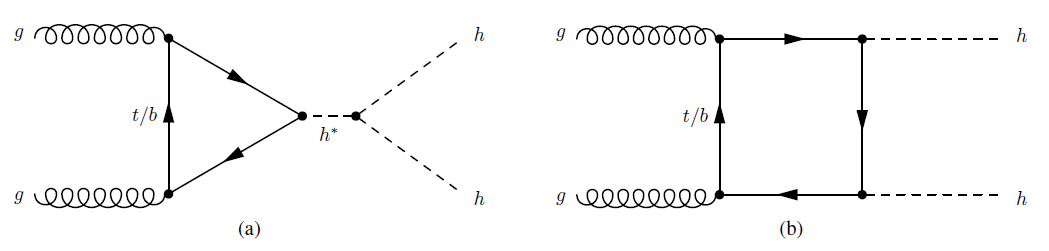
\includegraphics[width=0.9\textwidth]{figures/sm_nonres_hh_production}
    \caption{Representative diagrams that contribute to non-resonant \hh production.
    \textit{Left}: Diagram that is sensitive to the trilinear coupling, $\lambda$.
    \textit{Right}: Box diagram that interferese destructively with the $\lambda$-sensitive
    process.} 
    \label{fig:sm_nonres_hh}
\end{figure}


As a result of the destructive interference, and the already relatively large Higgs mass of
125 \GeV, the SM \dihiggs production has a total cross-section of $\sim 33.4$ fb ~\cite{CERN-YR-4}
at a \pp center-of-mass collision energy of 13 \TeV. The inclusive cross-section for the pair-production
of top quarks, which will be one of the dominant SM backgrounds in the present
analysis, is nearly 1000 pb, or $1\times10^6$ fb ~\cite{TOPQ-2015-09, ATLAS-CONF-2015-049}. That
of \textit{single} Higgs production is $\sim 50$ pb, or $5 \times 10^4$ fb ~\cite{ATLAS-CONF-2015-060}.

Furthermore, enhancements to the di-Higgs production rate, either non-resonantly or through a resonance, may be observable with the full Run2 dataset and would point to new physics beyond the Standard Model, making such analyses interesting now. The wide class of two Higgs double models (2HDM) predict an altered and enlarged
Higgs sector from which the currently Higgs is built.
The Minimal Supersymmetric Standard Model
(MSSM) is a  class of 2HDM. For the latter set, one such model is a Randall-Sundrum
type graviton or the lightest Kaluza-Klein excitation which have masses of at least
$2\times$ the mass of the SM Higgs boson. The presence of such BSM scenarios would act to alter
the measured value of $\lambda$ with respect to that of the SM, potentially enlarging it.
As a result, early evidence for the pair-production of Higgs bosons within the current
Run-2 dataset may indicate the presence of new physics without having to resort to
precision measurements of $\lambda$. Examples of such decay
scenarios are illustrated in example Feynman diagrams in Figure \ref{fig:2hdm_feynman_diagrams}.

\begin{figure}[!htb]
    \centering
    
\includegraphics[width=0.8\textwidth]{figures/mg5_hh_heavy_scalar.png}
    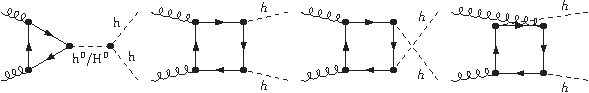
\includegraphics[width=0.8\textwidth]{figures/mg5_hh_2hdm_cp_even.png}
    \caption
    {
        Diagrams contributing to enhanced $hh$ production scenarios.
        \textit{Top}: A heavy scalar, $H$, that couples to the Standard Model Higgs
        boson, $h$, contributes to the Standard Model processes (left two diagrams).
        \textit{Bottom}: CP-even diagrams in 2HDM scenario that contribute to enhanced
        non-resonant production of Standard Model Higgs bosons as well as resonant
        channels with the heavy CP-even Higgs, $H^0$, decaying to the Standard Model
        low-mass CP-even Higgs, $h$.
    }
    \label{fig:2hdm_feynman_diagrams}
\end{figure}


In addition to the hh production mechanisms described above, the searches for evidence of an dditional extended Higgs sector model that introduces two new heavy Higgs bosons, X and S~\cite{vonBuddenbrock:2016rmr}. In this model, $X$ couples strongly to both $S$ and $h$. $S$ couples weakly to SM particles, suppressing direct production, but has the same mass-dependent branching ratios as $h$. 

Searches for resonant Higgs pair production have been performed in a number of final states, $b\bar{b}b\bar{b}$, $b\bar{b}\tau^{\pm}\tau^{\mp}$, $b\bar{b}\gamma\gamma$, $W^{\pm}W^{\mp *}\gamma\gamma$, $b\bar{b}VV$ (With $V$ either $Z$ or $W$) and $W^+W^-W^+W^-$ at $\sqrt{s}=8\,\TeV$ and $\sqrt{s}=13\,\TeV$ by ATLAS~\cite{HIGG-2013-33,Aad:2019uzh} and CMS collaborations~\cite{CMS-HIG-13-032,CMS-HIG-15-013,PhysRevLett.122.121803} including the combination of multiple final states. 

In this note, the searches for the \dihiggs non-resonant production in multilepton final states is described. Typically the decay modes of \dihiggs of $W^+W^-W^+W^-$, $ZZ^*bb$, $VV\tauh\tauh$, $\tauh\tauh\tauh\tauh$, $ZZZZ$ are the dominant ones which corresponds to 5.7\% of all \dihiggs decays. Additionally, $\gamma\gamma + X$ final states are studied which corresponds to 0.13\% of \dihiggs decays. Simple extension of the SM by introducing two new scalars $gg \rightarrow X \rightarrow SH$ signature is investigated.


This note is organised as follows: Section~\ref{sec:dataset} describes the Monte Carlo (MC) samples as well as the 
recorded dataset used in this analysis. The object definition and event preselection are detailed in Section~\ref{sec:objselec}. 
The signal region definitions and the multivariate analysis discriminants are described in Section~\ref{sec:eventselec}. 
The reducible background estimates using data-driven method are explained in Section~\ref{sec:nonpromptbkg}. 
%Section~\ref{sec:bkgval} shows the data and MC agreement of the prompt lepton background contributions in 
various validation regions.  
Theoretical and experimental systematic uncertainties are described in Section~\ref{sec:systematics}. 
An overview of the signal regions before the fit can be found in Section~\ref{sec:signalregion}.
Section~\ref{sec:results} describes the expected fit results for each individual channel and the 
expected and observed fit results for the combination. 
Finally, the conclusions are summarised in Section~\ref{sec:conclusion}.



